\chapter{Temporal-Difference Learning}
\label{ch:td}

\begin{quote}
\itshape
If one had to identify one idea as central and novel to reinforcement learning, it would undoubtedly be temporal-difference (TD) learning.
\end{quote}

\bigskip

Temporal-difference learning is the single most important idea in reinforcement learning.  It synthesises two powerful strands of thought: the \emph{sampling} approach of Monte Carlo methods, which learns directly from experience without a model of the environment, and the \emph{bootstrapping} approach of dynamic programming, which updates estimates on the basis of other estimates rather than waiting for the final outcome.  The result is a family of algorithms that can learn online, after every single transition, in both episodic and continuing tasks, without requiring a model of the environment.

This chapter develops the TD family in full generality.  We begin with the simplest member, TD(0), and establish its key properties: the TD error, its zero-mean property under the true value function, and convergence.  We then move to TD control algorithms\,---\,SARSA, Q-learning, Expected SARSA, and Double Q-learning\,---\,and carefully compare their on-policy and off-policy characters.  We generalise to $n$-step returns, which interpolate between TD and Monte Carlo, and then to the full TD($\lambda$) algorithm with eligibility traces, which combines information from all horizons simultaneously.  We conclude with Generalised Advantage Estimation (GAE), a modern technique for advantage estimation in policy gradient methods that is built squarely on the TD($\lambda$) machinery, and with a careful analysis of bias, variance, and convergence across the entire family.

% ===========================================================
\section{TD(0) Prediction}
\label{sec:td0}

\subsection{From Monte Carlo to Temporal Difference}

Recall from Chapter~\ref{ch:mc} that Monte Carlo (MC) prediction estimates the value function $V^\pi$ by averaging complete sample returns.  After each full episode, each visited state $S_t$ receives the update
\begin{equation}
\label{eq:mc-update}
V(S_t) \leftarrow V(S_t) + \alpha\bigl(G_t - V(S_t)\bigr),
\end{equation}
where $G_t = \sum_{k=0}^{\infty}\gamma^k R_{t+k+1}$ is the discounted return from time $t$.  This estimator is unbiased---$\E_\pi[G_t \mid S_t = s] = V^\pi(s)$---but it has three limitations: it requires the episode to terminate before any learning can occur; it accumulates reward variance over long horizons; and it cannot be applied to continuing (non-episodic) tasks at all.

The Bellman equation\index{Bellman equation} for a fixed policy $\pi$ offers an alternative target.  Because
\begin{equation}
\label{eq:bellman-v}
V^\pi(s) = \E_\pi\bigl[R_{t+1} + \gamma V^\pi(S_{t+1}) \mid S_t = s\bigr],
\end{equation}
the true value of state $s$ equals the expected immediate reward plus the discounted value of the next state.  Equation~\eqref{eq:bellman-v} is exact when $V = V^\pi$, but even with an imperfect estimate $V \approx V^\pi$ the quantity
\begin{equation}
\label{eq:td0-target}
R_{t+1} + \gamma V(S_{t+1})
\end{equation}
provides a useful \emph{one-step target}\index{one-step target} that can be computed as soon as the next transition $(S_t, A_t, R_{t+1}, S_{t+1})$ is observed.  Replacing the full return $G_t$ in~\eqref{eq:mc-update} with this one-step target yields

\begin{equation}
\label{eq:td0-update}
\boxed{V(S_t) \leftarrow V(S_t) + \alpha\Bigl(R_{t+1} + \gamma V(S_{t+1}) - V(S_t)\Bigr).}
\end{equation}
This is the \textbf{TD(0)}\index{TD(0)} algorithm, also called the one-step temporal-difference method.

\subsection{The TD Error}

\begin{definition}[TD error]
\label{def:td-error}
\index{TD error}
The \textbf{temporal-difference error} at time $t$ is
\begin{equation}
\label{eq:td-error}
\delta_t = R_{t+1} + \gamma V(S_{t+1}) - V(S_t).
\end{equation}
\end{definition}

The TD error measures the discrepancy between the current estimate $V(S_t)$ and the one-step target $R_{t+1}+\gamma V(S_{t+1})$.  With this notation, the TD(0) update~\eqref{eq:td0-update} simplifies to
\[
V(S_t) \leftarrow V(S_t) + \alpha\,\delta_t.
\]
The sign of $\delta_t$ has an immediate intuitive interpretation:
\begin{itemize}[leftmargin=*]
  \item $\delta_t > 0$: the observed transition was better than expected; $V(S_t)$ should be increased.
  \item $\delta_t < 0$: the state was overvalued; $V(S_t)$ should be decreased.
  \item $\delta_t = 0$: the current estimate is locally consistent with the Bellman equation.
\end{itemize}

\begin{definition}[Bootstrapping]
\label{def:bootstrap}
\index{bootstrapping}
\textbf{Bootstrapping} is the use of the current estimate of the value function as part of the target in the update rule.  In TD(0), the target $R_{t+1}+\gamma V(S_{t+1})$ depends on the estimate $V$ at the next state, so the method bootstraps.  Monte Carlo does not bootstrap because $G_t$ is the actual return, independent of $V$.
\end{definition}

\subsection{Zero-Mean Property of the TD Error}

The following result is fundamental: it shows that $\delta_t$ is a valid (zero-mean) gradient signal when the value function is exact.

\begin{theorem}[Zero mean of TD error]
\label{thm:td-error-zero-mean}
\index{TD error!zero-mean property}
If $V = V^\pi$, then for every state $s$,
\begin{equation}
\label{eq:td-zero-mean}
\E_\pi[\delta_t \mid S_t = s] = 0.
\end{equation}
\end{theorem}

\begin{proof}
Substituting $V = V^\pi$ into the definition~\eqref{eq:td-error},
\[
\delta_t = R_{t+1} + \gamma V^\pi(S_{t+1}) - V^\pi(S_t).
\]
Taking the conditional expectation given $S_t = s$:
\begin{align*}
\E_\pi[\delta_t \mid S_t = s]
&= \E_\pi\bigl[R_{t+1} + \gamma V^\pi(S_{t+1}) \mid S_t = s\bigr] - V^\pi(s)\\
&= V^\pi(s) - V^\pi(s) = 0,
\end{align*}
where the second line uses the Bellman equation~\eqref{eq:bellman-v}.
\end{proof}

Theorem~\ref{thm:td-error-zero-mean} implies that, at the fixed point, the TD update has zero expected change.  Before convergence, $\delta_t \ne 0$ on average, and its sign consistently points in the direction that reduces the Bellman error.

\subsection{TD(0) Algorithm}

\begin{algorithm}[ht]
\caption{TD(0) for Policy Evaluation}
\label{alg:td0}
\KwIn{Policy $\pi$, step size $\alpha\in(0,1]$, discount $\gamma\in[0,1)$}
Initialise $V(s) \leftarrow 0$ for all $s \in \cS$, $V(s_{\mathrm{term}}) \leftarrow 0$\;
\For{each episode}{
  Initialise $S_0$\;
  \For{$t = 0, 1, 2, \ldots$ until $S_t$ is terminal}{
    Choose $A_t \sim \pi(\cdot \mid S_t)$\;
    Take action $A_t$; observe $R_{t+1}$ and $S_{t+1}$\;
    $\delta_t \leftarrow R_{t+1} + \gamma V(S_{t+1}) - V(S_t)$\;
    $V(S_t) \leftarrow V(S_t) + \alpha\,\delta_t$\;
  }
}
\end{algorithm}

Note that, unlike Monte Carlo, the update at line~8 occurs \emph{immediately} after each transition\,---\,no waiting for the end of the episode.

\subsection{Convergence of Tabular TD(0)}

The convergence of TD(0) can be understood through the Bellman operator\index{Bellman operator} framework.  For a fixed policy $\pi$, define
\[
(T^\pi V)(s) = \E_\pi\bigl[R_{t+1} + \gamma V(S_{t+1}) \mid S_t = s\bigr].
\]
The Bellman equation reads $V^\pi = T^\pi V^\pi$.  Since $T^\pi$ is a $\gamma$-contraction in the supremum norm, its unique fixed point is $V^\pi$.  TD(0) can be interpreted as stochastic approximation of the iteration $V \leftarrow T^\pi V$: instead of computing the full expectation, it uses a single sample transition.

\begin{theorem}[Convergence of tabular TD(0)]
\label{thm:td0-convergence}
\index{TD(0)!convergence}
In the tabular setting, suppose $\pi$ is fixed, all states are visited infinitely often, rewards are bounded, and the step sizes $\{\alpha_t(s)\}$ satisfy the Robbins--Monro conditions\index{Robbins--Monro conditions}
\begin{equation}
\label{eq:rm-conditions}
\sum_{t=1}^{\infty}\alpha_t(s) = \infty, \qquad \sum_{t=1}^{\infty}\alpha_t^2(s) < \infty \quad \text{for each } s.
\end{equation}
Then $V_t(s) \to V^\pi(s)$ almost surely for all $s\in\cS$.
\end{theorem}

The Robbins--Monro conditions~\eqref{eq:rm-conditions} require that the step sizes are large enough for the algorithm to correct any initial error (first condition) but small enough for the noise to average out (second condition).  The schedule $\alpha_t(s) = 1/N_t(s)$, where $N_t(s)$ is the visit count, satisfies both conditions.  A constant step size $\alpha$ satisfies only the first, so it does not converge to the exact $V^\pi$ but tracks it in a non-stationary environment.

\subsection{Worked Example: Random Walk}

\begin{example}[Five-state random walk]
\label{ex:random-walk}
\index{random walk example}
Consider a five-state Markov chain with states $A, B, C, D, E$ arranged linearly, plus two terminal states $L$ (left) and $R$ (right).  From any non-terminal state, the agent moves left or right with equal probability $0.5$.  The only nonzero reward is $+1$ on the transition into the right terminal state $R$; all other rewards are $0$.  The discount factor is $\gamma = 1$.  The true state values (i.e.\ the probability of eventually reaching $R$) are
\[
V^\pi(A)=\tfrac{1}{6}, \quad V^\pi(B)=\tfrac{2}{6}, \quad V^\pi(C)=\tfrac{3}{6}, \quad V^\pi(D)=\tfrac{4}{6}, \quad V^\pi(E)=\tfrac{5}{6}.
\]
Suppose we initialise $V(s) = 0.5$ for all states and run TD(0) with $\alpha = 0.1$.  Consider a single trajectory that goes $C \to D \to E \to R$.

\textbf{Step 1}: $S_t = C$, $A_t = \text{right}$, $R_{t+1} = 0$, $S_{t+1} = D$.
\[
\delta_t = 0 + 1.0 \cdot 0.5 - 0.5 = 0.
\]
No update occurs this step (since $V(D) = V(C) = 0.5$ initially).

\textbf{Step 2}: $S_t = D$, $R_{t+1} = 0$, $S_{t+1} = E$.
\[
\delta_t = 0 + 0.5 - 0.5 = 0.
\]
Again no change.

\textbf{Step 3}: $S_t = E$, $R_{t+1} = 1$, $S_{t+1} = R$ (terminal, $V(R)=0$).
\[
\delta_t = 1 + 0 - 0.5 = 0.5.
\]
\[
V(E) \leftarrow 0.5 + 0.1 \times 0.5 = 0.55.
\]
The reward signal propagates only one step backward.  Over many episodes, TD(0) gradually propagates value estimates backward through the chain.  After approximately 100 episodes, the estimates are close to the true values.  This example demonstrates both the speed advantage of TD (learning within each episode) and the credit-assignment challenge: each new reward signal must propagate back through the state space visit by visit.
\end{example}

% ===========================================================
\section{Advantages of TD Methods}
\label{sec:td-advantages}

TD methods occupy a privileged position in the RL landscape because they inherit advantages from both Monte Carlo and dynamic programming while avoiding their main weaknesses.  We catalogue these advantages carefully.

\paragraph{No complete episode required.}
Monte Carlo methods must wait until the end of an episode to compute $G_t$.  This is problematic for long episodes and impossible for continuing tasks with no natural termination.  TD(0) updates after every single step, making it immediately applicable to any task structure.

\paragraph{Works for continuing tasks.}
Because the TD target $R_{t+1}+\gamma V(S_{t+1})$ is always available (no terminal state needed), TD methods naturally handle continuing tasks.  Monte Carlo methods cannot, in their basic form, be applied to such settings.

\paragraph{Lower variance than Monte Carlo.}
The Monte Carlo return $G_t = R_{t+1} + \gamma R_{t+2} + \gamma^2 R_{t+3} + \cdots$ accumulates variance from every future reward.  The TD target $R_{t+1}+\gamma V(S_{t+1})$ only involves one random reward and the (relatively smooth) estimate $V(S_{t+1})$.  Formally, if each reward has variance $\sigma^2$ and transitions are independent, the MC variance grows roughly as $\sum_{k=0}^{T-t-1} \gamma^{2k}\sigma^2$, whereas the TD variance is approximately $\sigma^2 + \gamma^2 \Var[V(S_{t+1})]$.

\paragraph{Bias--variance trade-off.}\index{bias--variance trade-off}
The price paid for lower variance is that the TD target is \emph{biased}: since $V \ne V^\pi$ early in training, the target $R_{t+1}+\gamma V(S_{t+1})$ does not equal $V^\pi(S_t)$ in expectation.  By Theorem~\ref{thm:td-error-zero-mean}, bias disappears at convergence.  Monte Carlo is unbiased but high-variance.  This fundamental trade-off\,---\,bootstrapping buys lower variance at the cost of bias\,---\,runs through all TD methods and is quantified in Section~\ref{sec:td-bias-variance}.

\paragraph{Faster credit assignment.}
Because TD propagates value estimates one step at a time within each episode, useful information from rewarding transitions is incorporated into earlier states more quickly than with MC.  $n$-step TD (Section~\ref{sec:nstep-td}) and eligibility traces (Section~\ref{sec:td-lambda}) provide mechanisms to propagate credit across multiple steps efficiently.

\paragraph{Batch TD(0) and the maximum likelihood estimate.}\index{batch TD(0)}
When a fixed batch of episodes is available, one can repeatedly apply TD(0) updates until convergence.  This \emph{batch TD(0)} converges to the \emph{maximum likelihood} (certainty-equivalence) estimate of $V^\pi$ given the data\,---\,the exact solution that would be computed by constructing the empirical MDP from the batch and solving it.  In contrast, batch Monte Carlo converges to the estimate that minimises the mean-squared error on the training returns.  In problems with limited data, the TD solution often generalises better because it exploits the Markov structure.

% ===========================================================
\section{SARSA: On-Policy TD Control}
\label{sec:sarsa}

\subsection{From Prediction to Control}

Policy evaluation tells us how good the current policy is.  Control requires we improve it.  As in Monte Carlo control (Chapter~\ref{ch:mc}), the key insight is to estimate the \emph{action-value function}\index{action-value function} $Q^\pi(s,a) = \E_\pi[G_t \mid S_t=s, A_t=a]$ rather than $V^\pi(s)$, because greedy improvement requires comparing actions:
\[
\pi'(s) \in \argmax_{a\in\cA}\; Q(s,a).
\]
The Bellman equation for $Q^\pi$ is
\begin{equation}
\label{eq:bellman-q}
Q^\pi(s,a) = \E_\pi\bigl[R_{t+1} + \gamma Q^\pi(S_{t+1},A_{t+1}) \mid S_t=s, A_t=a\bigr].
\end{equation}
Replacing the expectation in~\eqref{eq:bellman-q} by a single sample and applying the resulting update gives:

\subsection{The SARSA Update}

\begin{definition}[SARSA]
\label{def:sarsa}
\index{SARSA}
\textbf{SARSA}\footnote{The name stands for the five-tuple $(S_t, A_t, R_{t+1}, S_{t+1}, A_{t+1})$ used in each update.} (Rummery and Niranjan, 1994; Sutton, 1996) is the on-policy TD control algorithm with update rule
\begin{equation}
\label{eq:sarsa}
Q(S_t,A_t) \leftarrow Q(S_t,A_t) + \alpha\Bigl(R_{t+1} + \gamma Q(S_{t+1},A_{t+1}) - Q(S_t,A_t)\Bigr).
\end{equation}
\end{definition}

The critical feature of SARSA is that $A_{t+1}$ is drawn from the \emph{same} policy $\pi$ that is being used to collect data.  This makes SARSA \textbf{on-policy}\index{on-policy}: it evaluates and improves the policy that generates the data.

\begin{proposition}
The target $Y_t^{\mathrm{SARSA}} = R_{t+1} + \gamma Q(S_{t+1},A_{t+1})$ is an unbiased sample of the Bellman operator applied to $Q$:
\[
\E_\pi\bigl[Y_t^{\mathrm{SARSA}} \mid S_t=s, A_t=a\bigr] = (T^\pi Q)(s,a),
\]
where $(T^\pi Q)(s,a) = \E_\pi[R_{t+1}+\gamma Q(S_{t+1},A_{t+1}) \mid S_t=s, A_t=a]$.
\end{proposition}

\begin{proof}
By definition of the conditional expectation, the claim follows immediately.
\end{proof}

\begin{algorithm}[ht]
\caption{SARSA (On-Policy TD Control)}
\label{alg:sarsa}
\KwIn{Step size $\alpha$, discount $\gamma$, exploration $\varepsilon$}
Initialise $Q(s,a)$ for all $s,a$; $Q(s_{\mathrm{term}},\cdot)\leftarrow 0$\;
\For{each episode}{
  Initialise $S$\;
  Choose $A$ from $\pi(\cdot\mid S)$ derived from $Q$ (e.g.\ $\varepsilon$-greedy)\;
  \For{each step of episode until $S$ is terminal}{
    Take action $A$; observe $R, S'$\;
    Choose $A'$ from $\pi(\cdot\mid S')$ (same $\varepsilon$-greedy)\;
    $Q(S,A) \leftarrow Q(S,A) + \alpha\bigl(R + \gamma Q(S',A') - Q(S,A)\bigr)$\;
    $S \leftarrow S'$;\quad $A \leftarrow A'$\;
  }
}
\end{algorithm}

\subsection{Convergence of SARSA}

\begin{theorem}[Convergence of SARSA]
\index{SARSA!convergence}
In the tabular setting, SARSA converges to $Q^*$ almost surely if: (1) all state-action pairs are visited infinitely often; (2) the policy converges to the greedy policy (e.g.\ $\varepsilon_t \to 0$); and (3) the step sizes satisfy the Robbins--Monro conditions~\eqref{eq:rm-conditions}.
\end{theorem}

The convergence requires the policy to become greedy in the limit, so exploration must be reduced over time.  In practice, constant $\varepsilon$ or constant $\alpha$ are often used, in which case SARSA converges to a neighbourhood of $Q^*$ rather than to $Q^*$ exactly.

\subsection{Worked Example: Cliff Walking}

\begin{example}[Cliff Walking]
\label{ex:cliff-walking}
\index{Cliff Walking}
Consider a $4 \times 12$ gridworld with a cliff along the bottom edge (cells $(3,1)$ through $(3,10)$).  The agent starts at $(3,0)$ and must reach the goal at $(3,11)$.  Stepping onto the cliff gives reward $-100$ and returns the agent to start.  All other transitions give reward $-1$.  Episodes terminate at the goal or after 200 steps.

SARSA with $\varepsilon=0.1$ learns the \emph{safe path} along the top of the grid, staying far from the cliff.  Because the exploratory actions occasionally push the agent toward the cliff, SARSA evaluates the cliff cells as dangerous and avoids them.  Q-learning (Section~\ref{sec:q-learning}), being off-policy, evaluates each state under the \emph{greedy} policy and therefore discovers the shortest path along the cliff edge\,---\,but this path is fragile in practice because $\varepsilon$-greedy exploration sometimes causes it to fall into the cliff during training.  This is the canonical illustration of the on-policy/off-policy trade-off: SARSA is safer during learning; Q-learning finds the theoretically optimal policy.
\end{example}

% ===========================================================
\section{Q-Learning: Off-Policy TD Control}
\label{sec:q-learning}

\subsection{The Q-Learning Update}

Q-learning (Watkins, 1989)\index{Q-learning} directly approximates the optimal action-value function $Q^*$ by using the Bellman \emph{optimality} equation as its target.  Since $Q^*(s,a) = \E[R_{t+1}+\gamma\max_{a'}Q^*(S_{t+1},a') \mid S_t=s,A_t=a]$, a single-sample approximation gives

\begin{equation}
\label{eq:q-learning}
\boxed{Q(S_t,A_t) \leftarrow Q(S_t,A_t) + \alpha\Bigl(R_{t+1} + \gamma\max_{a'} Q(S_{t+1},a') - Q(S_t,A_t)\Bigr).}
\end{equation}

The key difference from SARSA~\eqref{eq:sarsa} is the \textbf{max} operator.  No matter how $A_{t+1}$ is actually chosen (whether by $\varepsilon$-greedy or any other behaviour policy), the target always uses the greedy action in $S_{t+1}$.  This makes Q-learning \textbf{off-policy}\index{off-policy}: the behaviour policy collects data, but the update evaluates the greedy (target) policy.

\begin{algorithm}[ht]
\caption{Q-Learning (Off-Policy TD Control)}
\label{alg:q-learning}
\KwIn{Step size $\alpha$, discount $\gamma$, exploration $\varepsilon$}
Initialise $Q(s,a)$ for all $s,a$; $Q(s_{\mathrm{term}},\cdot)\leftarrow 0$\;
\For{each episode}{
  Initialise $S$\;
  \For{each step until $S$ is terminal}{
    Choose $A$ from $Q$ using $\varepsilon$-greedy\;
    Take action $A$; observe $R, S'$\;
    $Q(S,A) \leftarrow Q(S,A) + \alpha\bigl(R + \gamma\max_{a'}Q(S',a') - Q(S,A)\bigr)$\;
    $S \leftarrow S'$\;
  }
}
\end{algorithm}

\subsection{Convergence of Q-Learning}

\begin{theorem}[Convergence of Q-learning, Watkins and Dayan 1992]
\label{thm:q-learning-convergence}
\index{Q-learning!convergence}
In a finite MDP, if all state-action pairs are visited infinitely often, rewards are bounded, and the step sizes satisfy the Robbins--Monro conditions~\eqref{eq:rm-conditions}, then Q-learning converges to $Q^*$ almost surely.
\end{theorem}

This result is remarkable: it holds regardless of the behaviour policy used to generate transitions, as long as every $(s,a)$ pair is visited sufficiently often.  Q-learning is thus a fully off-policy method with convergence guarantees in the tabular case.

\subsection{Maximisation Bias}
\label{subsec:max-bias}
\index{maximisation bias}

A subtle but important problem arises from using $\max_{a'} Q(S_{t+1},a')$ as a target.  When $Q$ is an estimate with noise, the maximum over noisy values is a \emph{positively biased} estimator of the true maximum value.  This is because, by Jensen's inequality applied to the convex max function,
\[
\E\!\left[\max_{a'}Q(S_{t+1},a')\right] \ge \max_{a'}\E[Q(S_{t+1},a')].
\]
The bias can be substantial when there are many actions with similar true values but noisy estimates.

\begin{example}[Maximisation bias]
Suppose state $s'$ has three actions with true values $Q^*(s',a_1)=Q^*(s',a_2)=Q^*(s',a_3)=0$.  Estimates $\hat Q(s',a_i)\sim\cN(0,\sigma^2)$ are independent Gaussian noise.  Then $\E[\max_i\hat Q(s',a_i)] > 0$, a positive bias that grows with $\sigma^2$ and with the number of actions.  Q-learning uses this biased maximum as a target, causing systematic overestimation.
\end{example}

% ===========================================================
\section{Expected SARSA}
\label{sec:expected-sarsa}

\index{Expected SARSA}
SARSA uses the actual next action $A_{t+1}$ in its target, introducing variance from the policy's randomness.  Q-learning eliminates this variance by taking the greedy action, but incurs maximisation bias.  \textbf{Expected SARSA} (van Seijen et al., 2009) takes the middle path: it replaces $Q(S_{t+1},A_{t+1})$ with the \emph{expectation} over the policy:

\begin{equation}
\label{eq:expected-sarsa}
Q(S_t,A_t) \leftarrow Q(S_t,A_t) + \alpha\Biggl(R_{t+1} + \gamma\sum_{a'}\pi(a'\mid S_{t+1})\,Q(S_{t+1},a') - Q(S_t,A_t)\Biggr).
\end{equation}

\begin{algorithm}[ht]
\caption{Expected SARSA}
\label{alg:expected-sarsa}
\KwIn{Step size $\alpha$, discount $\gamma$, policy $\pi$ (or $\varepsilon$-greedy)}
Initialise $Q(s,a)$ for all $s,a$\;
\For{each episode}{
  Initialise $S$\;
  \For{each step until $S$ is terminal}{
    Choose $A$ from $\pi(\cdot\mid S)$\;
    Take action $A$; observe $R,S'$\;
    Compute $\bar Q(S') \leftarrow \sum_{a'}\pi(a'\mid S')\,Q(S',a')$\;
    $Q(S,A) \leftarrow Q(S,A) + \alpha\bigl(R + \gamma\,\bar Q(S') - Q(S,A)\bigr)$\;
    $S \leftarrow S'$\;
  }
}
\end{algorithm}

Expected SARSA eliminates the variance from the random choice of $A_{t+1}$, so its updates are less noisy than SARSA's.  It can also be used off-policy: if $\pi$ is the greedy policy (probability 1 on $\argmax_a Q(s,a)$, probability 0 elsewhere), Expected SARSA reduces exactly to Q-learning, since
\[
\sum_{a'}\pi_{\mathrm{greedy}}(a'\mid s')Q(s',a') = \max_{a'}Q(s',a').
\]
Thus Expected SARSA generalises both SARSA (on-policy, $\pi$ is the behaviour policy) and Q-learning (off-policy, $\pi$ is greedy).

% ===========================================================
\section{Double Q-Learning}
\label{sec:double-q}

\index{Double Q-learning}
Double Q-learning (van Hasselt, 2010) addresses maximisation bias by maintaining \emph{two independent} action-value estimates, $Q_1$ and $Q_2$.  The idea is to \emph{decouple} action selection from action evaluation:
\begin{itemize}[leftmargin=*]
  \item Use $Q_1$ to select the greedy action: $a^* = \argmax_{a'} Q_1(S_{t+1},a')$.
  \item Use $Q_2$ to evaluate that action: target $= R_{t+1} + \gamma Q_2(S_{t+1},a^*)$.
\end{itemize}
Since $Q_1$ and $Q_2$ are independent estimates, using one to select and the other to evaluate removes the upward bias.  Crucially, the roles of $Q_1$ and $Q_2$ are swapped with probability $0.5$ at each step to keep both estimates up to date.

\begin{algorithm}[ht]
\caption{Double Q-Learning}
\label{alg:double-q}
\KwIn{Step size $\alpha$, discount $\gamma$, exploration $\varepsilon$}
Initialise $Q_1(s,a)$ and $Q_2(s,a)$ for all $s,a$\;
\For{each episode}{
  Initialise $S$\;
  \For{each step until $S$ is terminal}{
    $A \leftarrow \varepsilon$-greedy w.r.t.\ $Q_1(S,\cdot)+Q_2(S,\cdot)$\;
    Observe $R,S'$\;
    \eIf{with probability $0.5$}{
      $a^* \leftarrow \argmax_{a'}Q_1(S',a')$\;
      $Q_1(S,A) \leftarrow Q_1(S,A) + \alpha\bigl(R+\gamma Q_2(S',a^*)-Q_1(S,A)\bigr)$\;
    }{
      $a^* \leftarrow \argmax_{a'}Q_2(S',a')$\;
      $Q_2(S,A) \leftarrow Q_2(S,A) + \alpha\bigl(R+\gamma Q_1(S',a^*)-Q_2(S,A)\bigr)$\;
    }
    $S \leftarrow S'$\;
  }
}
\end{algorithm}

Double Q-learning provably reduces maximisation bias and performs better than Q-learning in environments with many actions.  The idea was later scaled to deep RL in the Double DQN algorithm (van Hasselt, Guez, and Silver, 2016), which uses the online network for action selection and the target network for evaluation.

% ===========================================================
\section{Comparison: SARSA, Q-Learning, and Expected SARSA}
\label{sec:td-control-comparison}

Table~\ref{tab:td-control-comparison} summarises the three main TD control algorithms.

\begin{table}[ht]
\centering
\caption{Comparison of on-policy and off-policy TD control algorithms.}
\label{tab:td-control-comparison}
\small
\begin{tabular}{@{}lccc@{}}
\toprule
\textbf{Property} & \textbf{SARSA} & \textbf{Q-Learning} & \textbf{Expected SARSA}\\
\midrule
Target & $R\!+\!\gamma Q(S',A')$ & $R\!+\!\gamma\max_{a'}Q(S',a')$ & $R\!+\!\gamma\!\sum_{a'}\pi(a'|S')Q(S',a')$\\
Policy & On-policy & Off-policy & Both\\
Goal & $Q^\pi$ & $Q^*$ & $Q^\pi$ or $Q^*$\\
Variance & Medium & Low & Lower than SARSA\\
Bias & Unbiased & Max.~bias & Unbiased\\
Safe? & Yes & No (cliff) & Yes\\
\bottomrule
\end{tabular}
\end{table}

\begin{figure}[ht]
\centering
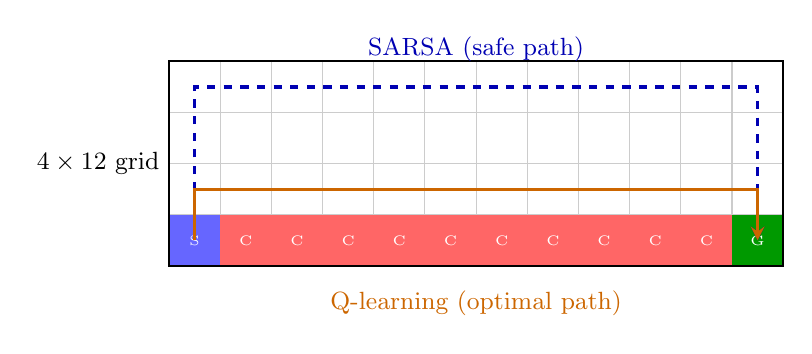
\begin{tikzpicture}[x=0.65cm, y=0.65cm, >=stealth]
  % Draw the grid
  \foreach \x in {0,...,11} {
    \foreach \y in {0,...,3} {
      \draw[gray!40] (\x,\y) rectangle (\x+1,\y+1);
    }
  }
  % Cliff cells (bottom row, columns 1-10)
  \foreach \x in {1,...,10} {
    \fill[red!60] (\x,0) rectangle (\x+1,1);
    \node[font=\tiny,white] at (\x+0.5,0.5) {C};
  }
  % Start
  \fill[blue!60] (0,0) rectangle (1,1);
  \node[font=\tiny,white] at (0.5,0.5) {S};
  % Goal
  \fill[green!60!black] (11,0) rectangle (12,1);
  \node[font=\tiny,white] at (11.5,0.5) {G};
  % Grid border
  \draw[thick] (0,0) rectangle (12,4);
  % SARSA path (along top)
  \draw[->, very thick, blue!70!black, dashed]
    (0.5,0.5) -- (0.5,3.5) -- (11.5,3.5) -- (11.5,0.5);
  \node[blue!70!black,font=\small,above] at (6,3.8) {SARSA (safe path)};
  % Q-learning path (along cliff edge)
  \draw[->, very thick, orange!80!black]
    (0.5,0.5) -- (0.5,1.5) -- (11.5,1.5) -- (11.5,0.5);
  \node[orange!80!black,font=\small,below] at (6,-0.3) {Q-learning (optimal path)};
  % Labels
  \node[left,font=\small] at (0,2) {$4\times 12$ grid};
\end{tikzpicture}
\caption{Cliff Walking gridworld.  The red cells are the cliff (reward $-100$, reset to start).  SARSA (dashed blue) learns a safe path along the top; Q-learning (solid orange) learns the theoretically shorter path along the cliff edge but is fragile under $\varepsilon$-greedy exploration.}
\label{fig:cliff-walking}
\end{figure}

The Cliff Walking example (Example~\ref{ex:cliff-walking} and Figure~\ref{fig:cliff-walking}) illustrates the practical consequence of on-policy vs.\ off-policy evaluation.  During training with $\varepsilon$-greedy exploration, SARSA accounts for the possibility of random actions pushing it into the cliff and therefore prefers the safer route.  Q-learning evaluates states under the greedy policy\,---\,which never steps off the cliff\,---\,so it learns the cliff-edge route, which is optimal but fragile.  At test time ($\varepsilon=0$) both find equivalent paths, but SARSA achieves higher average reward during learning.

% ===========================================================
\section{$n$-Step TD Methods}
\label{sec:nstep-td}

\subsection{The $n$-Step Return}

Both TD(0) and Monte Carlo are special cases of a more general family parameterised by the \emph{lookahead horizon} $n\in\{1,2,\dots\}$.  The \textbf{$n$-step return}\index{n-step return} is defined as

\begin{equation}
\label{eq:nstep-return}
G_t^{(n)} = R_{t+1} + \gamma R_{t+2} + \cdots + \gamma^{n-1}R_{t+n} + \gamma^n V(S_{t+n}),
\end{equation}
and the corresponding update is
\begin{equation}
\label{eq:nstep-update}
V(S_t) \leftarrow V(S_t) + \alpha\bigl(G_t^{(n)} - V(S_t)\bigr).
\end{equation}

\begin{proposition}
The $n$-step return satisfies:
\begin{enumerate}
  \item At $n=1$: $G_t^{(1)} = R_{t+1}+\gamma V(S_{t+1})$, the TD(0) target.
  \item In an episodic task with terminal time $T$: $G_t^{(T-t)} = G_t$, the full Monte Carlo return (using $V(S_T)=0$).
\end{enumerate}
\end{proposition}

\begin{proof}
(1) Setting $n=1$ in~\eqref{eq:nstep-return} gives $G_t^{(1)} = R_{t+1}+\gamma V(S_{t+1})$.  (2) With $n=T-t$ and $V(S_T)=0$: $G_t^{(T-t)} = \sum_{k=0}^{T-t-1}\gamma^k R_{t+k+1} = G_t$.
\end{proof}

\subsection{Bias--Variance Trade-Off in $n$-Step TD}

As $n$ increases, the $n$-step return interpolates between the biased-but-low-variance TD(0) target and the unbiased-but-high-variance MC return:
\begin{itemize}[leftmargin=*]
  \item Small $n$: more bootstrapping, higher bias, lower variance.
  \item Large $n$: less bootstrapping, lower bias, higher variance.
\end{itemize}
The optimal $n$ depends on the problem: in environments with dense, low-variance rewards, small $n$ works well; in sparse-reward environments, larger $n$ is often beneficial.

\begin{figure}[ht]
\centering
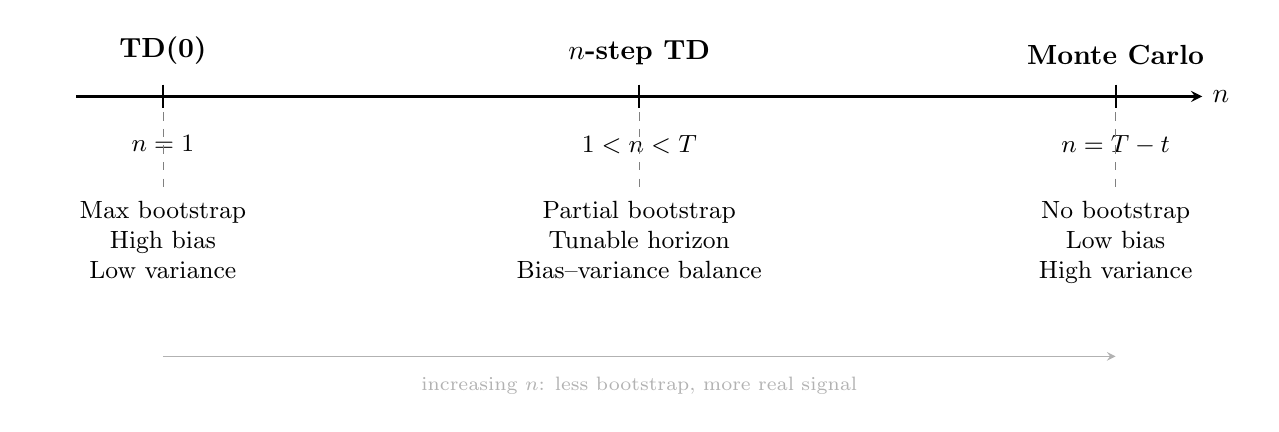
\begin{tikzpicture}[x=1.1cm, y=1cm, >=stealth,
    box/.style={align=center, font=\small, text width=3.2cm}]
  \draw[->, thick] (0,0) -- (13,0) node[right] {$n$};
  \foreach \x/\lbl in {1/{$n=1$}, 6.5/{$1<n<T$}, 12/{$n=T-t$}}{
    \draw[thick] (\x,0.15) -- (\x,-0.15) node[below=6pt,font=\small]{\lbl};
  }
  \node[above=8pt,font=\bfseries] at (1,0) {TD(0)};
  \node[above=8pt,font=\bfseries] at (6.5,0) {$n$-step TD};
  \node[above=8pt,font=\bfseries] at (12,0) {Monte Carlo};
  \node[box, below=1.2cm] at (1,0)   {Max bootstrap\\High bias\\Low variance};
  \node[box, below=1.2cm] at (6.5,0) {Partial bootstrap\\Tunable horizon\\Bias--variance balance};
  \node[box, below=1.2cm] at (12,0)  {No bootstrap\\Low bias\\High variance};
  \draw[very thin, gray, dashed] (1,-0.2) -- (1,-1.15);
  \draw[very thin, gray, dashed] (6.5,-0.2) -- (6.5,-1.15);
  \draw[very thin, gray, dashed] (12,-0.2) -- (12,-1.15);
  \draw[->,gray!60] (1,-3.3) -- (12,-3.3)
    node[midway,below=4pt,font=\scriptsize,align=center]{increasing $n$: less bootstrap, more real signal};
\end{tikzpicture}
\caption{The spectrum of $n$-step TD methods.  TD(0) ($n=1$) and Monte Carlo ($n=T-t$) are the extreme cases.  Intermediate $n$ provides a bias--variance trade-off that can be tuned to the task.}
\label{fig:nstep-spectrum}
\end{figure}

\subsection{$n$-Step SARSA}

The $n$-step idea extends naturally to control.  The $n$-step SARSA target is
\[
G_t^{(n)} = R_{t+1} + \gamma R_{t+2} + \cdots + \gamma^{n-1}R_{t+n} + \gamma^n Q(S_{t+n},A_{t+n}),
\]
and the update is $Q(S_t,A_t) \leftarrow Q(S_t,A_t)+\alpha(G_t^{(n)}-Q(S_t,A_t))$.  This algorithm shares convergence guarantees with standard SARSA under appropriate conditions.

% ===========================================================
\section{TD($\lambda$) and Eligibility Traces}
\label{sec:td-lambda}

The $n$-step methods of the previous section require fixing a single horizon $n$ in advance.  TD($\lambda$) instead combines \emph{all} $n$-step returns simultaneously, weighting them geometrically so that the combined target is computable online with a single extra vector, the \emph{eligibility trace}.

\subsection{The $\lambda$-Return}

\begin{definition}[$\lambda$-return]
\label{def:lambda-return}
\index{lambda-return@$\lambda$-return}
For $\lambda\in[0,1]$, the \textbf{$\lambda$-return} is the geometrically weighted average of all $n$-step returns:
\begin{equation}
\label{eq:lambda-return}
G_t^\lambda = (1-\lambda)\sum_{n=1}^{\infty}\lambda^{n-1}G_t^{(n)}.
\end{equation}
\end{definition}

The weight given to the $n$-step return is $(1-\lambda)\lambda^{n-1}$.  These weights are positive, decrease geometrically with $n$, and sum to one:
\[
\sum_{n=1}^{\infty}(1-\lambda)\lambda^{n-1} = (1-\lambda)\cdot\frac{1}{1-\lambda} = 1.
\]
Thus $G_t^\lambda$ is a genuine convex combination of the $n$-step returns.

\paragraph{Special cases.}
\begin{itemize}[leftmargin=*]
  \item $\lambda = 0$: $G_t^0 = G_t^{(1)} = R_{t+1}+\gamma V(S_{t+1})$, the TD(0) target.  All weight is on the one-step return.
  \item $\lambda = 1$: $G_t^1 = G_t$, the complete Monte Carlo return.  The geometric weights are flat (all equal to zero for finite $n$; the limit equals the full return).
\end{itemize}
Thus TD($\lambda$) subsumes both TD(0) and Monte Carlo as extreme cases, just as $n$-step TD does\,---\,but with an elegant, differentiable interpolation.

% \begin{figure}[ht]
% \centering
% \begin{tikzpicture}[x=0.7cm, y=2.5cm, >=stealth]
%   % Draw weight bars for different lambdas
%   \def\lam{0.6}
%   % Title
%   \node[font=\small\bfseries] at (6.5,1.05) {$\lambda$-return weights $(1-\lambda)\lambda^{n-1}$ for $\lambda=0.6$};
%   % Bars
%   \foreach \n in {1,...,12}{
%     \pgfmathsetmacro\w{(1-\lam)*(\lam^(\n-1))}
%     \pgfmathsetmacro\wscaled{\w*5}
%     \fill[blue!50!white] (\n-0.4,0) rectangle (\n+0.4,\wscaled);
%     \draw[blue!70!black] (\n-0.4,0) rectangle (\n+0.4,\wscaled);
%   }
%   % Axes
%   \draw[->,thick] (0.5,0) -- (13.5,0) node[right,font=\small] {$n$};
%   \draw[->,thick] (0.5,0) -- (0.5,1.0) node[above,font=\small] {weight};
%   % Tick labels
%   \foreach \n in {1,2,3,4,5,6,7,8,9,10,11,12}{
%     \draw ({\n},0.02) -- ({\n},-0.02);
%     \node[below,font=\tiny] at (\n,-0.02) {$\n$};
%   }
%   % y ticks
%   \foreach \y/\lbl in {0.2/0.08, 0.5/0.20, 1.0/0.40}{
%     \draw (0.4,\y) -- (0.6,\y);
%     \node[left,font=\tiny] at (0.4,\y) {\lbl};
%   }
% \end{tikzpicture}
% \caption{Weights $(1-\lambda)\lambda^{n-1}$ assigned to each $n$-step return in the $\lambda$-return ($\lambda=0.6$).  Short-horizon returns receive the most weight; the weights decay geometrically, so the influence of distant returns diminishes rapidly.}
% \label{fig:lambda-weights}
% \end{figure}

\begin{figure}[ht]
\centering
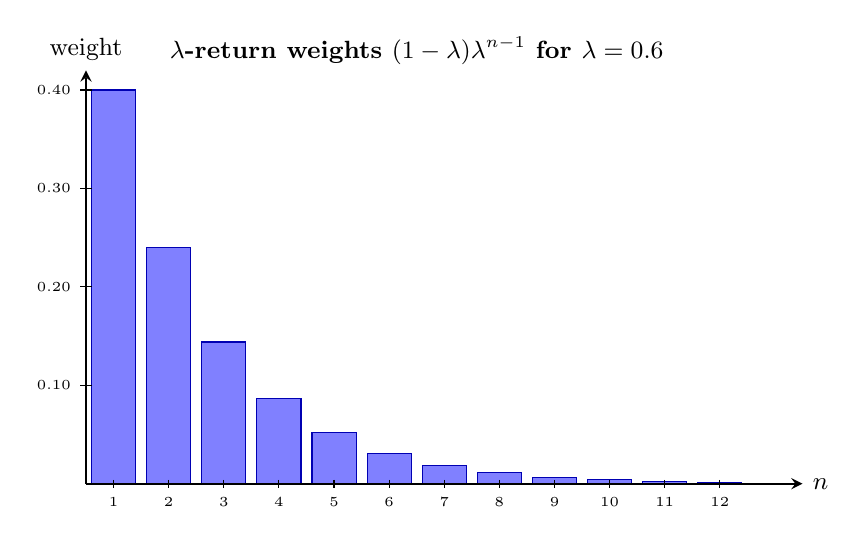
\begin{tikzpicture}[x=0.7cm, y=2.5cm, >=stealth]
  % Draw weight bars for different lambdas
  \def\lam{0.6}
  % Title
  \node[font=\small\bfseries] at (6.5,2.2) {$\lambda$-return weights $(1-\lambda)\lambda^{n-1}$ for $\lambda=0.6$};
  % Bars
  \foreach \n in {1,...,12}{
    \pgfmathsetmacro\w{(1-\lam)*(\lam^(\n-1))}
    \pgfmathsetmacro\wscaled{\w*5}
    \fill[blue!50!white] (\n-0.4,0) rectangle (\n+0.4,\wscaled);
    \draw[blue!70!black] (\n-0.4,0) rectangle (\n+0.4,\wscaled);
  }
  % Axes
  \draw[->,thick] (0.5,0) -- (13.5,0) node[right,font=\small] {$n$};
  \draw[->,thick] (0.5,0) -- (0.5,2.1) node[above,font=\small] {weight};
  % Tick labels
  \foreach \n in {1,2,3,4,5,6,7,8,9,10,11,12}{
    \draw ({\n},0.02) -- ({\n},-0.02);
    \node[below,font=\tiny] at (\n,-0.02) {$\n$};
  }
  % y ticks
  \foreach \y/\lbl in {0.5/0.10, 1.0/0.20, 1.5/0.30, 2.0/0.40}{
    \draw (0.4,\y) -- (0.6,\y);
    \node[left,font=\tiny] at (0.4,\y) {\lbl};
  }
\end{tikzpicture}
\caption{Weights $(1-\lambda)\lambda^{n-1}$ assigned to each $n$-step return in the $\lambda$-return ($\lambda=0.6$).  Short-horizon returns receive the most weight; the weights decay geometrically, so the influence of distant returns diminishes rapidly.}
\label{fig:lambda-weights}
\end{figure}

\subsection{Forward View of TD($\lambda$)}
\label{subsec:forward-view}
\index{TD(lambda)!forward view}

The \textbf{forward view} of TD($\lambda$) defines the update target for state $S_t$ as $G_t^\lambda$ and applies
\[
V(S_t) \leftarrow V(S_t) + \alpha\bigl(G_t^\lambda - V(S_t)\bigr).
\]
This is conceptually clean: the target is a specific, well-defined quantity.  However, computing $G_t^\lambda$ requires the entire future trajectory from time $t$, so the forward view requires waiting until the episode terminates before any update can be applied.  It is therefore not online in the operational sense, and it is equivalent to a single-pass post-hoc update over the episode.

Despite its impracticality for online learning, the forward view is the \emph{gold standard} for understanding what TD($\lambda$) computes.  The backward view, which we develop next, is mathematically equivalent to the forward view but operates online.

\subsection{Eligibility Traces}
\label{subsec:eligibility-traces}
\index{eligibility trace}

The key to making TD($\lambda$) online is the \textbf{eligibility trace}\index{eligibility trace} $e_t(s)$, a vector over states that records how ``eligible'' each state is for a credit update at time $t$.

\begin{definition}[Eligibility trace (accumulating)]
\label{def:elig-trace}
The \textbf{accumulating eligibility trace} for state $s$ is initialised to $e_0(s)=0$ and updated each step by
\begin{equation}
\label{eq:elig-trace}
e_t(s) = \gamma\lambda\, e_{t-1}(s) + \ind\{S_t = s\}.
\end{equation}
\end{definition}

The trace $e_t(s)$ increases by 1 each time state $s$ is visited and decays by factor $\gamma\lambda$ at every time step.  Intuitively, it measures the recency and frequency of visits to $s$: a state visited frequently and recently has a high trace.

An alternative is the \textbf{replacing eligibility trace}\index{eligibility trace!replacing}:
\begin{equation}
\label{eq:elig-trace-replacing}
e_t(s) = \begin{cases} \gamma\lambda\, e_{t-1}(s) + 1 & \text{if } s = S_t,\\ \gamma\lambda\, e_{t-1}(s) & \text{otherwise,}\end{cases}
\quad\text{capped at 1.}
\end{equation}
Replacing traces prevent the trace for the current state from exceeding 1, which can stabilise learning in some settings.

\subsection{Backward View of TD($\lambda$): The Online Algorithm}
\label{subsec:backward-view}
\index{TD(lambda)!backward view}

In the \textbf{backward view}, a single TD error $\delta_t$ is computed each step, and \emph{all} states are updated simultaneously, weighted by their eligibility traces:

\begin{equation}
\label{eq:td-lambda-update}
\boxed{V(s) \leftarrow V(s) + \alpha\,\delta_t\,e_t(s), \quad \forall s\in\cS.}
\end{equation}

The TD error $\delta_t = R_{t+1}+\gamma V(S_{t+1})-V(S_t)$ is broadcast to all states, but only states with a nonzero trace receive a meaningful update.  Recently visited states\,---\,which have high traces\,---\,receive large updates; states not visited recently have near-zero traces and are barely affected.  This is the ``credit assignment'' mechanism of eligibility traces: good or bad outcomes are credited proportionally to the recency and frequency of past visits.

\begin{algorithm}[ht]
\caption{TD($\lambda$) with Eligibility Traces}
\label{alg:td-lambda}
\KwIn{Step size $\alpha$, discount $\gamma$, trace parameter $\lambda$}
Initialise $V(s)\leftarrow 0$ for all $s$\;
\For{each episode}{
  $e(s) \leftarrow 0$ for all $s$\;
  Initialise $S$\;
  \For{each step $t$ until $S$ is terminal}{
    Choose $A\sim\pi(\cdot\mid S)$; observe $R, S'$\;
    $\delta \leftarrow R + \gamma V(S') - V(S)$\;
    $e(S) \leftarrow e(S) + 1$ \quad(accumulating trace)\;
    \For{all $s\in\cS$}{
      $V(s) \leftarrow V(s) + \alpha\,\delta\,e(s)$\;
      $e(s) \leftarrow \gamma\lambda\,e(s)$\;
    }
    $S \leftarrow S'$\;
  }
}
\end{algorithm}

In practice, only states with nonzero traces need to be updated, so the inner loop over all $s$ is typically replaced by maintenance of an active-trace set.  The algorithm requires $O(|\cS|)$ memory per episode\,---\,one trace value per state.

\subsection{Equivalence of Forward and Backward Views}

The following theorem is the cornerstone of the eligibility trace theory.

\begin{theorem}[Forward--backward equivalence of TD($\lambda$)]
\label{thm:fb-equivalence}
\index{TD(lambda)!forward-backward equivalence}
For the offline (end-of-episode) updating version of TD($\lambda$) with constant step size $\alpha$, the sum of all updates made to $V(s)$ during an episode is identical under the forward view and the backward view.  That is, defining $\Delta_t V(s) = \alpha(G_t^\lambda - V(S_t))\ind\{S_t=s\}$ (forward) and $\Delta_t^{\mathrm{bw}}V(s) = \alpha\delta_t e_t(s)$ (backward):
\begin{equation}
\label{eq:fb-equiv}
\sum_{t=0}^{T-1}\Delta_t^{\mathrm{bw}}V(s) = \sum_{t=0}^{T-1}\Delta_t V(s), \quad \forall s\in\cS.
\end{equation}
\end{theorem}

\begin{proof}[Proof sketch]
The key identity is
\[
G_t^\lambda - V(S_t) = \sum_{k=t}^{T-1}(\gamma\lambda)^{k-t}\delta_k,
\]
which expresses the $\lambda$-return error as a discounted sum of future TD errors.  To verify this, expand $G_t^\lambda$ using the definition~\eqref{eq:lambda-return}, write each $G_t^{(n)}$ as a telescoping sum of TD errors (using $G_t^{(n)} = \delta_t + \gamma G_{t+1}^{(n-1)}$ recursively), then collect terms.  The full algebraic derivation can be found in Sutton \& Barto (2018, Chapter 12).

Once this identity is established, summing $\alpha\delta_t e_t(s)$ over $t$ and exchanging the order of summation gives $\sum_t \alpha(G_t^\lambda-V(S_t))\ind\{S_t=s\}$, completing the proof.
\end{proof}

Theorem~\ref{thm:fb-equivalence} confirms that the online, incremental backward view computes exactly the same updates as the offline forward view.  This is a profound result: it means we do not have to choose between conceptual clarity (forward) and computational efficiency (backward).

\subsection{Practical Considerations}

\begin{remark}[Trace decay and effective horizon]
The product $\gamma\lambda$ controls the effective decay rate of eligibility traces.  For $\gamma\lambda = 0.9$, a state visited $k$ steps ago has trace $0.9^k$, so states visited more than $\sim 20$ steps ago have negligible trace.  Practitioners often tune $\lambda$ jointly with $\gamma$ to set the desired effective horizon.
\end{remark}

\begin{remark}[Computational cost]
The naive implementation of Algorithm~\ref{alg:td-lambda} updates all $|\cS|$ traces at each step, which is $O(|\cS|)$ per step.  With tabular representations this is feasible for moderate state spaces.  With function approximation (Chapter~\ref{ch:value-approx}), the trace becomes a vector of the same dimension as the parameter vector, and the per-step cost is $O(d)$ where $d$ is the number of parameters.
\end{remark}

\begin{remark}[SARSA($\lambda$) and Q($\lambda$)]
Eligibility traces extend naturally to control.  \textbf{SARSA($\lambda$)}\index{SARSA(lambda)@SARSA($\lambda$)} maintains a trace $e_t(s,a)$ over state-action pairs and uses the SARSA TD error $\delta_t = R_{t+1}+\gamma Q(S_{t+1},A_{t+1})-Q(S_t,A_t)$ to update $Q(s,a) \leftarrow Q(s,a)+\alpha\delta_t e_t(s,a)$.  Similarly, \textbf{Q($\lambda$)}\index{Q(lambda)@Q($\lambda$)} applies the Q-learning TD error with traces.  SARSA($\lambda$) is particularly popular in practice because it maintains the on-policy nature of SARSA while incorporating the multi-step credit assignment of eligibility traces.
\end{remark}

\subsection{Worked Example: Random Walk with TD($\lambda$)}

\begin{example}[Effect of $\lambda$ on learning speed]
Return to the five-state random walk of Example~\ref{ex:random-walk}.  Running TD($\lambda$) with various values of $\lambda$ for a fixed number of episodes and measuring the RMS error relative to the true values, we observe:
\begin{itemize}[leftmargin=*]
  \item $\lambda=0$ (TD(0)): learns slowly; reward signal takes many episodes to propagate to distant states.
  \item $\lambda=0.5$: traces ensure that a reward obtained at the right terminal propagates backward to states visited in the last several steps within the same episode, substantially accelerating learning.
  \item $\lambda=0.9$: fast early learning but slightly more noisy, since traces give significant weight to distant states that may not have contributed to the final reward.
  \item $\lambda=1$ (MC): slowest per-episode variance is high, but with a well-tuned step size, total learning across episodes can be competitive.
\end{itemize}
In Sutton and Barto's experiments, intermediate values $\lambda\approx 0.7$--$0.9$ often achieve the lowest RMS error for this task.  The optimal $\lambda$ depends on the step size and the task structure.
\end{example}

% ===========================================================
\section{Generalised Advantage Estimation (GAE)}
\label{sec:gae}

\index{Generalised Advantage Estimation (GAE)}
\index{advantage function}
Generalised Advantage Estimation (Schulman et al., 2016) is a modern technique for computing low-variance advantage estimates for use in policy gradient methods (Chapter~\ref{ch:pg}).  It is built directly on the TD($\lambda$) machinery and provides a compelling application of the theory developed in this chapter.

\subsection{The Advantage Function}

\begin{definition}[Advantage function]
\label{def:advantage}
\index{advantage function}
The \textbf{advantage function} of policy $\pi$ is
\begin{equation}
\label{eq:advantage}
A^\pi(s,a) = Q^\pi(s,a) - V^\pi(s).
\end{equation}
\end{definition}

The advantage $A^\pi(s,a)$ measures how much better action $a$ is in state $s$ compared to the average action under policy $\pi$.  By definition:
\begin{itemize}[leftmargin=*]
  \item $A^\pi(s,a) > 0$: action $a$ is better than average; the policy should increase the probability of $a$.
  \item $A^\pi(s,a) < 0$: action $a$ is worse than average; decrease its probability.
  \item $A^\pi(s,a) = 0$: action $a$ performs exactly at the average.
\end{itemize}
Note that $\E_{a\sim\pi(\cdot|s)}[A^\pi(s,a)] = 0$ for all $s$, so the advantage is centred.

\paragraph{Why advantage matters for policy gradients.}
The policy gradient theorem (Chapter~\ref{ch:pg}) states that the gradient of the expected return with respect to the policy parameters $\theta$ is
\[
\nabla_\theta J(\theta) = \E_\pi\bigl[\nabla_\theta\log\pi_\theta(A_t\mid S_t)\cdot\Psi_t\bigr],
\]
where $\Psi_t$ can be the return $G_t$, the action-value $Q^\pi(S_t,A_t)$, or\,---\,crucially\,---\,the advantage $A^\pi(S_t,A_t)$.  Using the advantage instead of the raw return or action-value dramatically reduces variance: the baseline $V^\pi(S_t)$ is subtracted, removing all variation due to the state (which the policy cannot influence).

\subsection{$n$-Step Advantage Estimates}

In practice, $V^\pi$ and $A^\pi$ are unknown.  Given a learned critic $V_\phi \approx V^\pi$, a natural estimator of the one-step advantage is the TD error:
\begin{equation}
\label{eq:td-advantage}
\hat A_t^{(1)} = \delta_t = R_{t+1} + \gamma V_\phi(S_{t+1}) - V_\phi(S_t).
\end{equation}
More generally, the $n$-step advantage estimate is
\begin{equation}
\label{eq:nstep-advantage}
\hat A_t^{(n)} = \sum_{l=0}^{n-1}\gamma^l R_{t+l+1} + \gamma^n V_\phi(S_{t+n}) - V_\phi(S_t).
\end{equation}
Note that $\hat A_t^{(n)} = G_t^{(n)} - V_\phi(S_t)$, where $G_t^{(n)}$ is the $n$-step return~\eqref{eq:nstep-return}.

\subsection{GAE: The $\lambda$-Weighted Advantage}

\begin{definition}[Generalised Advantage Estimation]
\label{def:gae}
\index{GAE}
The \textbf{Generalised Advantage Estimation} $\hat A_t^{\mathrm{GAE}(\gamma,\lambda)}$ is the exponentially weighted average of $n$-step advantage estimates:
\begin{equation}
\label{eq:gae}
\hat A_t^{\mathrm{GAE}(\gamma,\lambda)} = \sum_{l=0}^{\infty}(\gamma\lambda)^l\,\delta_{t+l},
\end{equation}
where $\delta_{t+l} = R_{t+l+1} + \gamma V_\phi(S_{t+l+1}) - V_\phi(S_{t+l})$ is the TD error at time $t+l$.
\end{definition}

\begin{proposition}
GAE is a $\lambda$-weighted average of $n$-step advantage estimates:
\begin{equation}
\label{eq:gae-lambda-avg}
\hat A_t^{\mathrm{GAE}(\gamma,\lambda)} = (1-\lambda)\sum_{n=1}^{\infty}\lambda^{n-1}\hat A_t^{(n)}.
\end{equation}
\end{proposition}

\begin{proof}
We use the key identity $\hat A_t^{(n)} = \sum_{l=0}^{n-1}(\gamma)^l\delta_{t+l}$ (telescoping), which follows from
\[
\hat A_t^{(n)} = \sum_{l=0}^{n-1}\gamma^l R_{t+l+1} + \gamma^n V_\phi(S_{t+n}) - V_\phi(S_t)
= \sum_{l=0}^{n-1}\gamma^l\delta_{t+l}.
\]
Then
\begin{align*}
(1-\lambda)\sum_{n=1}^{\infty}\lambda^{n-1}\hat A_t^{(n)}
&= (1-\lambda)\sum_{n=1}^{\infty}\lambda^{n-1}\sum_{l=0}^{n-1}\gamma^l\delta_{t+l}\\
&= (1-\lambda)\sum_{l=0}^{\infty}\gamma^l\delta_{t+l}\sum_{n=l+1}^{\infty}\lambda^{n-1}\\
&= (1-\lambda)\sum_{l=0}^{\infty}\gamma^l\delta_{t+l}\cdot\frac{\lambda^l}{1-\lambda}\\
&= \sum_{l=0}^{\infty}(\gamma\lambda)^l\delta_{t+l}.
\end{align*}
\end{proof}

\subsection{Special Cases and Bias--Variance Trade-Off}

\begin{itemize}[leftmargin=*]
  \item $\lambda = 0$: $\hat A_t^{\mathrm{GAE}(\gamma,0)} = \delta_t = R_{t+1}+\gamma V_\phi(S_{t+1})-V_\phi(S_t)$.  This is the one-step TD advantage\,---\,lowest variance, highest bias (relies entirely on $V_\phi$).
  \item $\lambda = 1$: $\hat A_t^{\mathrm{GAE}(\gamma,1)} = \sum_{l=0}^{\infty}\gamma^l\delta_{t+l} = G_t - V_\phi(S_t)$.  This is the Monte Carlo advantage estimate\,---\,lowest bias, highest variance.
  \item Intermediate $\lambda$: exponentially decaying weights average short-horizon (low-variance, high-bias) and long-horizon (high-variance, low-bias) estimates.
\end{itemize}

\subsection{Connection to TD($\lambda$)}

The structure of GAE~\eqref{eq:gae} is identical to the $\lambda$-return mechanism.  In fact, if we view $V_\phi(S_t)$ as a baseline, then
\[
\hat A_t^{\mathrm{GAE}(\gamma,\lambda)} = G_t^\lambda - V_\phi(S_t),
\]
where $G_t^\lambda$ is the $\lambda$-return computed with the critic $V_\phi$.  Thus GAE is simply the TD($\lambda$) target minus the current value estimate.  The eligibility trace view provides an efficient way to compute GAE online: maintain a trace $e_t$ and accumulate $e_t\,\delta_t$ terms.

In practice (e.g.\ in the PPO and TRPO algorithms), GAE is computed in a backward pass over a collected rollout of length $T$:
\begin{align*}
A_T &= 0,\\
A_t &= \delta_t + \gamma\lambda\,A_{t+1}, \quad t = T-1, T-2, \ldots, 0,
\end{align*}
which is a linear recursion that can be computed in $O(T)$ time.

\begin{example}[GAE computation on a short rollout]
Suppose $\gamma=0.99$, $\lambda=0.95$, and a rollout of 4 steps yields TD errors $\delta_0=0.5,\;\delta_1=-0.3,\;\delta_2=0.8,\;\delta_3=0.1$ (with $A_4=0$).  The backward computation gives:
\begin{align*}
A_3 &= 0.1 + 0 = 0.1,\\
A_2 &= 0.8 + 0.99\times 0.95\times 0.1 = 0.8 + 0.094 = 0.894,\\
A_1 &= -0.3 + 0.99\times 0.95\times 0.894 = -0.3 + 0.840 = 0.540,\\
A_0 &= 0.5 + 0.99\times 0.95\times 0.540 = 0.5 + 0.508 = 1.008.
\end{align*}
The advantage estimate $A_0 = 1.008$ for the first step accounts not only for $\delta_0 = 0.5$ but also for the downstream positive signal $\delta_2 = 0.8$, appropriately discounted by $(\gamma\lambda)^2$.
\end{example}

% ===========================================================
\section{Bias, Variance, and Convergence Analysis}
\label{sec:td-bias-variance}

\subsection{Formal Bias Analysis}

The TD(0) target $R_{t+1}+\gamma V_t(S_{t+1})$ is biased whenever $V_t \ne V^\pi$.  We can decompose the bias as follows.  Let $V_t$ denote the value estimate at iteration~$t$ and let $b_t(s) = V_t(s) - V^\pi(s)$ denote the approximation error at iteration~$t$.  Then
\begin{align*}
\E_\pi[R_{t+1}+\gamma V_t(S_{t+1})\mid S_t=s]
&= V^\pi(s) + \gamma\,\E_\pi[b_t(S_{t+1})\mid S_t=s],
\end{align*}
So the bias of the TD target equals $\gamma$ times the expected approximation error at the next state.  This is strictly smaller than the approximation error at $s$ in magnitude (scaled by $\gamma < 1$), which is the mechanism by which TD updates are pulled toward $V^\pi$.  As $V_t\to V^\pi$, the bias vanishes, consistent with Theorem~\ref{thm:td-error-zero-mean}.

Monte Carlo, on the other hand, uses the unbiased target $G_t$, so its bias is zero regardless of $V_t$.

\subsection{Variance Analysis}

The variance of the TD(0) target $R_{t+1}+\gamma V(S_{t+1})$ is bounded by
\[
\Var[R_{t+1}+\gamma V(S_{t+1})\mid S_t=s] \le \sigma_R^2 + \gamma^2\,\Var[V(S_{t+1})\mid S_t=s],
\]
where $\sigma_R^2$ is the reward variance.  When $V$ is a smooth function (e.g.\ a neural network), $\Var[V(S_{t+1})]$ is small.  In contrast, the MC return $G_t = \sum_{k=0}^{\infty}\gamma^k R_{t+k+1}$ accumulates variance from every step.  Since rewards at different time steps are generally correlated through the shared trajectory, the full expression includes cross-covariance terms:
\[
\Var[G_t\mid S_t=s] = \sum_{k=0}^{\infty}\gamma^{2k}\Var[R_{t+k+1}\mid S_t=s] + 2\!\!\sum_{0\le j<k}\!\!\gamma^{j+k}\Cov[R_{t+j+1},R_{t+k+1}\mid S_t=s] \;\gg\; \Var[R_{t+1}+\gamma V(S_{t+1})].
\]
This variance gap grows with episode length and discount, making TD methods substantially more sample-efficient than MC in many practical settings.

\subsection{Mean Squared Error Decomposition}

For any estimator $\hat y$ of a target $y^* = \E[Y]$, the mean squared error decomposes as
\begin{equation}
\label{eq:bias-variance-decomp}
\mathrm{MSE}(\hat y) = \underbrace{\bigl(\E[\hat y] - y^*\bigr)^2}_{\mathrm{Bias}^2} + \underbrace{\Var[\hat y]}_{\mathrm{Variance}}.
\end{equation}
This decomposition applies to the TD target (biased, low variance) and the MC return (unbiased, high variance).  Minimising MSE requires balancing both terms, which is precisely what TD($\lambda$) does by tuning $\lambda$.

\subsection{Comparison Table}

\begin{table}[ht]
\centering
\caption{Bias, variance, and convergence properties of prediction methods.}
\label{tab:bias-variance-comparison}
\begin{tabular}{lcccc}
\toprule
\textbf{Method} & \textbf{Bias} & \textbf{Variance} & \textbf{Online?} & \textbf{Convergence}\\
\midrule
Monte Carlo & Zero & High (grows with $T$) & No & Yes (to $V^\pi$)\\
TD(0) & High early, $\to 0$ & Low & Yes & Yes (Thm.~\ref{thm:td0-convergence})\\
$n$-step TD & Medium & Medium & Semi & Yes\\
TD($\lambda$) & Tunable ($\lambda$) & Tunable ($\lambda$) & Yes & Yes\\
\bottomrule
\end{tabular}
\end{table}

\subsection{The Deadly Triad}
\index{deadly triad}

Tabular TD methods are guaranteed to converge under mild conditions.  However, combining three ingredients leads to potential divergence:
\begin{enumerate}
  \item \textbf{Function approximation} (e.g.\ linear or neural network representations of $V$).
  \item \textbf{Bootstrapping} (TD updates using the current estimate as a target).
  \item \textbf{Off-policy training} (learning from data generated by a different policy).
\end{enumerate}
This combination\,---\,known as the \emph{deadly triad}\,---\,can cause the value estimates to diverge to infinity even in simple linear examples (Baird's counterexample, 1995).  Monte Carlo avoids the triad by not bootstrapping; on-policy methods avoid it by staying on-policy; some algorithms (e.g.\ gradient TD methods, emphatic TD) address it through careful algorithmic design.  Chapter~\ref{ch:value-approx} treats these issues in depth.

\subsection{Convergence Under the Robbins--Monro Schedule}

The Robbins--Monro conditions~\eqref{eq:rm-conditions} are necessary for almost-sure convergence of stochastic approximation algorithms.  Their intuition is as follows:
\begin{itemize}[leftmargin=*]
  \item The divergence condition $\sum_t\alpha_t = \infty$ ensures the algorithm can correct any initial error, no matter how large.
  \item The square-summability condition $\sum_t\alpha_t^2 < \infty$ ensures accumulated noise is suppressed: the variance of the sum $\sum_t\alpha_t\epsilon_t$ (where $\epsilon_t$ is noise) is bounded by $\sigma^2\sum_t\alpha_t^2 < \infty$.
\end{itemize}
The harmonic schedule $\alpha_t = 1/t$ satisfies both conditions.  The constant schedule $\alpha_t = \alpha$ satisfies neither\,---\,leading to persistent fluctuations\,---\,but is often preferred in non-stationary problems or when rapid adaptation to distribution shifts is needed.

% ===========================================================
\section{Summary}
\label{sec:td-summary}

Temporal-difference learning unifies the Monte Carlo and dynamic programming traditions.  From the single idea of bootstrapping\,---\,using current value estimates as targets\,---\,an entire family of efficient, online, model-free algorithms emerges.  Table~\ref{tab:td-summary} provides a comprehensive overview of all methods introduced in this chapter.

\begin{table}[ht]
\centering
\caption{Summary of temporal-difference methods introduced in this chapter.}
\label{tab:td-summary}
\begin{tabular}{llllll}
\toprule
\textbf{Algorithm} & \textbf{Type} & \textbf{Policy} & \textbf{Target} & \textbf{Online} & \textbf{Credit}\\
\midrule
TD(0) & Prediction & Fixed $\pi$ & $R+\gamma V(S')$ & Yes & 1 step\\
$n$-step TD & Prediction & Fixed $\pi$ & $G^{(n)}$ & Semi & $n$ steps\\
TD($\lambda$) & Prediction & Fixed $\pi$ & $G^\lambda$ & Yes & Traces\\
SARSA & Control & On-policy & $R+\gamma Q(S',A')$ & Yes & 1 step\\
SARSA($\lambda$) & Control & On-policy & $G^\lambda_Q$ & Yes & Traces\\
Q-learning & Control & Off-policy & $R+\gamma\max_{a'}Q(S',a')$ & Yes & 1 step\\
Expected SARSA & Control & Both & $R+\gamma\bar Q(S')$ & Yes & 1 step\\
Double Q-learning & Control & Off-policy & Decoupled max & Yes & 1 step\\
\bottomrule
\end{tabular}
\end{table}

The key insights of this chapter are:
\begin{itemize}[leftmargin=*]
  \item The TD error $\delta_t = R_{t+1}+\gamma V(S_{t+1})-V(S_t)$ is the fundamental credit signal in RL; it has zero mean at convergence (Theorem~\ref{thm:td-error-zero-mean}).
  \item TD methods trade bias for variance: bootstrapping introduces bias but reduces variance compared to Monte Carlo.
  \item SARSA is on-policy and safe during exploration; Q-learning is off-policy and learns the optimal policy directly.
  \item TD($\lambda$) with eligibility traces elegantly bridges the gap between one-step TD and Monte Carlo, with the forward and backward views provably equivalent.
  \item GAE applies the $\lambda$-return machinery to advantage estimation in policy gradient methods, providing a clean bias--variance trade-off parameterised by $\lambda$.
  \item Convergence in the tabular setting is well understood; the combination of function approximation, bootstrapping, and off-policy data (the deadly triad) can cause divergence.
\end{itemize}


% ===========================================================
\section*{Exercises}
\addcontentsline{toc}{section}{Exercises}

\begin{exercise}
\label{ex:td-error-basic}
Suppose $V(S_t)=3$, $R_{t+1}=1$, $\gamma=0.9$, and $V(S_{t+1})=4$.
\begin{enumerate}[label=(\alph*)]
  \item Compute the TD error $\delta_t$.
  \item Apply one TD(0) update with step size $\alpha=0.1$.  What is the new value $V(S_t)$?
  \item Interpret the sign of $\delta_t$: was the state overvalued or undervalued?
\end{enumerate}
\end{exercise}

\begin{exercise}
\label{ex:td-error-zero-mean}
Let $V = V^\pi$ be the exact value function.  Provide a detailed proof that $\E_\pi[\delta_t \mid S_t=s]=0$ for all $s$, explicitly stating at which step you use the Bellman equation for $V^\pi$.  Then explain why this property does \emph{not} hold when $V \ne V^\pi$.
\end{exercise}

\begin{exercise}
\label{ex:sarsa-vs-qlearn}
Consider the Cliff Walking environment of Example~\ref{ex:cliff-walking}.
\begin{enumerate}[label=(\alph*)]
  \item Explain in precise terms why SARSA with $\varepsilon=0.1$ prefers the path far from the cliff, even though the cliff-edge path is shorter.
  \item Q-learning with $\varepsilon=0.1$ eventually learns the cliff-edge route.  If we decrease $\varepsilon$ to $0.01$, how does this affect (i) the path learned by Q-learning, and (ii) the path learned by SARSA?
  \item At test time with $\varepsilon=0$, which algorithm would you prefer, and why?
\end{enumerate}
\end{exercise}

\begin{exercise}
\label{ex:max-bias}
Consider a two-action MDP where the true $Q^*(s,a_1)=Q^*(s,a_2)=0$.  Let $\hat Q(s,a_i)\sim\cN(0,\sigma^2)$ be independent noisy estimates.
\begin{enumerate}[label=(\alph*)]
  \item Show that $\E[\max(\hat Q(s,a_1),\hat Q(s,a_2))]>0$.  (Hint: use the formula for the expected maximum of two standard normal random variables and scale by $\sigma$.)
  \item How does this bias grow as the number of actions increases?
  \item Explain how Double Q-learning (Algorithm~\ref{alg:double-q}) eliminates this bias.
\end{enumerate}
\end{exercise}

\begin{exercise}
\label{ex:nstep-returns}
For the five-state random walk of Example~\ref{ex:random-walk}, initialise all $V(s)=0.5$ and suppose the trajectory $B\to C\to D\to E\to R$ is observed with rewards $(0,0,0,1)$ and $\gamma=1$.
\begin{enumerate}[label=(\alph*)]
  \item Compute the TD(0) target ($n=1$) for state $B$.
  \item Compute the 2-step return $G_0^{(2)}$ for state $B$.
  \item Compute the full Monte Carlo return $G_0$ for state $B$.
  \item For the $\lambda$-return with $\lambda=0.5$, compute $G_0^\lambda$ for state $B$ (include all $n$-step terms).
\end{enumerate}
\end{exercise}

\begin{exercise}
\label{ex:elig-trace-compute}
In a tabular problem, a trajectory visits states $A, B, A, C$ at times $t=0,1,2,3$.  Using accumulating eligibility traces~\eqref{eq:elig-trace} with $\gamma=0.9$ and $\lambda=0.8$, compute the trace $e_t(s)$ for each state $s\in\{A,B,C\}$ at each time $t=0,1,2,3$.  Verify that at $t=3$, the trace $e_3(A)$ is larger than $e_3(B)$ because $A$ was visited twice and most recently.
\end{exercise}

\begin{exercise}
\label{ex:td-lambda-equiv}
State the forward--backward equivalence theorem (Theorem~\ref{thm:fb-equivalence}) in your own words.  Then use the identity $G_t^\lambda - V(S_t) = \sum_{k=t}^{T-1}(\gamma\lambda)^{k-t}\delta_k$ to verify the equivalence for a specific two-step episode: states $S_0, S_1, S_2$ (terminal), with rewards $R_1, R_2$ and discount $\gamma$.  Confirm that $\sum_{t=0}^{1}\alpha\,\delta_t\,e_t(S_0)$ equals $\alpha(G_0^\lambda - V(S_0))$.
\end{exercise}

\begin{exercise}
\label{ex:gae-compute}
Suppose $\gamma=0.99$, $\lambda=0.9$, and a trajectory of length 5 yields TD errors $\delta_0=1, \delta_1=0, \delta_2=-1, \delta_3=2, \delta_4=0$.
\begin{enumerate}[label=(\alph*)]
  \item Compute $\hat A_t^{\mathrm{GAE}(\gamma,\lambda)}$ for $t=0,1,2,3$ using the backward recursion from Section~\ref{sec:gae}.
  \item What would the estimates be if $\lambda=0$?  If $\lambda=1$?
  \item Interpret the difference: for which value of $\lambda$ does the advantage estimate at $t=0$ most strongly reflect the positive signal $\delta_3=2$?
\end{enumerate}
\end{exercise}

\begin{exercise}
\label{ex:deadly-triad}
The \emph{deadly triad} refers to the combination of bootstrapping, function approximation, and off-policy training.
\begin{enumerate}[label=(\alph*)]
  \item Explain why removing any one of the three elements restores convergence guarantees.
  \item Monte Carlo with function approximation is not known to diverge.  Which element of the triad is missing?
  \item On-policy TD with linear function approximation converges to a neighbourhood of $V^\pi$.  Which element of the triad is missing?
  \item Propose one algorithm design choice that retains all three elements while attempting to restore convergence.
\end{enumerate}
\end{exercise}

\begin{exercise}
\label{ex:rm-conditions}
Consider the step size schedule $\alpha_t = c/(t+t_0)$ for constants $c>0$ and $t_0>0$.
\begin{enumerate}[label=(\alph*)]
  \item Show that this schedule satisfies the Robbins--Monro conditions~\eqref{eq:rm-conditions}.
  \item Show that the constant schedule $\alpha_t = \alpha$ does \emph{not} satisfy the second condition.
  \item In a non-stationary environment where $V^\pi$ changes over time, explain why a constant step size is often \emph{preferred} despite lacking the second Robbins--Monro condition.
\end{enumerate}
\end{exercise}

\begin{exercise}
\label{ex:expected-sarsa-reduce}
Show algebraically that when the policy $\pi$ in Expected SARSA~\eqref{eq:expected-sarsa} is the deterministic greedy policy with respect to $Q$---i.e.\ $\pi(a\mid s) = \ind\{a = \argmax_{a'}Q(s,a')\}$---the Expected SARSA update reduces exactly to the Q-learning update~\eqref{eq:q-learning}.
\end{exercise}

\begin{exercise}
\label{ex:bias-variance-table}
Fill in the following table for a simple episodic task with average episode length $T=100$ and reward variance $\sigma^2=1$ per step.  Assume $\gamma=0.99$.  Estimate (order of magnitude) the variance of the update target for: (a) TD(0), (b) 10-step TD, (c) Monte Carlo.  Use the approximation that the $n$-step return variance is $\sum_{k=0}^{n-1}\gamma^{2k}\sigma^2 + \gamma^{2n}\Var[V(S_n)]$ and that $\Var[V(S_n)]\approx 0$ (perfect critic).  Discuss how the bias terms change as $n$ increases.
\end{exercise}
